\documentclass[UFT8]{beamer}
\usepackage{tikz}
\usetikzlibrary{arrows, positioning, shapes.geometric, arrows.meta}

\mode<presentation> {
	\usetheme{Frankfurt}
	% or AnnArbor Antibes Bergen Berkeley Berlin Boadilla boxes CambridgeUS Copenhagen Darmstadt default Dresden Frankfurt Goettingen Hannover Ilmenau JuanLesPinsLuebeck Madrid Malmoe Marburg Montpellier PaloAlto Pittsburgh Rochester Singapore Szeged Warsaw
	
	\setbeamercovered{transparent}
	% or whatever (possibly just delete it)
}

\usepackage{color}
\usepackage{algorithm,algpseudocode}
\usepackage{algorithmicx}
\usepackage{algpseudocode}
\usepackage{amsmath}
\usepackage{float}
\usepackage{bbm}

\usefonttheme[onlymath]{serif}

% \documentclass[ppt.tex]{subfiles}
\begin{document}

\section{{Assumptions}}

\begin{frame}
    \frametitle{DL, CDH}
	\begin{definition}[DL assumption]
		Given a generator $g$ of $\mathbb{G}$, and $a \in_R \mathbb{Z}_p$, for every adversary $\mathcal{A}$.
		$\Pr[\mathcal{A}(g, g^a) = a] \le \epsilon(\kappa)$
	\end{definition}

	\begin{definition}[CDH assumption]
		$a, b \in_R \mathbb{Z}_p$, for every adversary $\mathcal{A}$, $\Pr[\mathcal{A}(g, g^a, g^b) = g^{ab}] \le \epsilon(\kappa)$
	\end{definition}
\end{frame}

\begin{frame}
	\frametitle{Binding property of Pedersen Commitment}
	\begin{itemize}
		\item Setup: $h, u \leftarrow \mathbb{G}$
		\item Commit: $Com(x, r) = h^x u^r$
	\end{itemize}
	
	\begin{theorem}
		\begin{equation*}
			\Pr[a_1, a_2 \leftarrow \mathcal{A}(\mathbb{G}, h, u) : \exists a_i \neq 0 \land h^{a_1} u^{a_2} = 1] \le \epsilon(\kappa)
		\end{equation*}
	\end{theorem}

	\quad

	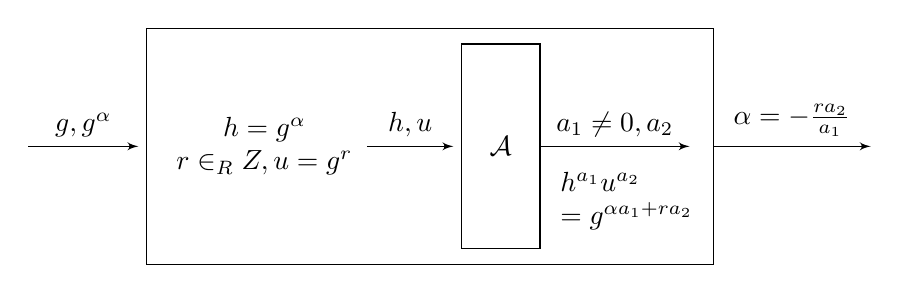
\begin{tikzpicture}[auto, node distance=2.5cm,>=latex']
        \draw[->] (-1.5, 1.5) -- node {$g, g^{\alpha}$} (-0.1, 1.5);
		\draw (0,0) rectangle (7.2,3);

		\node[align=center] at (1.5, 1.5) {$h=g^\alpha$ \\ $r \in_R \mathbb{Z}, u = g^r$};
        \draw[->] (2.8, 1.5) -- node {$h, u$} (3.9, 1.5);

		\node at (4.5, 1.5) {$\mathcal{A}$};
		\draw (4,0.2) rectangle (5,2.8);
        \draw[->] (5, 1.5) -- node {$a_1 \neq 0, a_2$} (6.9, 1.5);
		
		\node[align=left] at (6.1, 0.8) {$h^{a_1}u^{a_2}$ \\ $= g^{\alpha a_1 + r a_2}$};
		
        \draw[->] (7.2, 1.5) -- node {$\alpha = - \frac{ra_2}{a_1}$} (9.2, 1.5);
	\end{tikzpicture}
\end{frame}

\begin{frame}
	\frametitle{$t$-polyDH, $t$-SDH}
	\begin{definition}[$t$-polyDH]
		Let $\alpha \in_R \mathbb{Z}$. For every adversary $\mathcal{A}$,
		\begin{equation*}
			\Pr\left[\mathcal{A}\left(g, g^\alpha, \cdots, g^{\alpha^t}\right) = \langle \phi(x), g^{\phi(\alpha)} \rangle\right] \le \epsilon(\kappa)
		\end{equation*}
		for any freely chosen $\phi(x) \in \mathbb{Z}[X]$ such that $\deg(\phi) > t$.
	\end{definition}

	\begin{definition}[$t$-SDH Assumption]
		Let $\alpha \in_R \mathbb{Z}_p$. For every adversary $\mathcal{A}$,
		\begin{equation*}
			\Pr\left[\mathcal{A}\left(g, g^\alpha, \cdots, g^{\alpha^t} \right) = \langle c, g^{\frac{1}{\alpha + c}} \rangle \right] \le \epsilon(\kappa)
		\end{equation*}
		for any $c \in \mathbb{Z}$
	\end{definition}

\end{frame}

\begin{frame}
    \frametitle{$t$-BSDH}
	\begin{definition}[Bilinear Map]
		Let $\mathbb{G}_1, \mathbb{G}_2$ and $\mathbb{G}_t$ be cyclic groups of the same order.
		$e: \mathbb{G}_1 \times \mathbb{G}_2 \rightarrow \mathbb{G}_t$ such that for all $u \in \mathbb{G}_1, v \in \mathbb{G}_2, a, b \in \mathbb{Z}$
		$$
		e(u^a, v^b) = e(u, v)^{ab}
		$$
		Normally, $\mathbb{G}_1 = \mathbb{G}_2$, denote by $\mathbb{G}$.
	\end{definition}

	\begin{definition}[$t$-BSDH]
		Let $\alpha \in_R \mathbb{Z}_p$. For every adversary $\mathcal{A}$,
		\begin{equation*}
			\Pr\left[\mathcal{A}\left(g, g^\alpha, \cdots, g^{\alpha^t} \right) = \langle c, e(g, g)^{\frac{1}{\alpha + c}} \rangle \right] \le \epsilon(\kappa)
		\end{equation*}
		for any $c \in \mathbb{Z}$
	\end{definition}
\end{frame}

\begin{frame}
	\frametitle{KZG polynomial commitment scheme}

	\begin{itemize}
		\item $Setup(t) \rightarrow \left(g, g^\alpha, \cdots, g^{\alpha^t} \right) = pp$
		\item $Com(f(X), pp) \rightarrow g^{f(\alpha)} = \mathcal{C}$
		\item $Eval(f(X), z) \rightarrow g^{h(\alpha)} = \pi$, where $h(X) = \frac{f(X) - f(z)}{X - z}$
		\item $Verify(\mathcal{C}, z, f(z), \pi) \rightarrow b \in \{0, 1\}$. When 
		$$
		e\left(g, g^{f(\alpha) - f(z)} \right) = e\left(g^{\alpha - z}, g^{h(\alpha)}\right)
		$$
		$b=1$, otherwise $b = 0$.
		\begin{theorem}
			$Eval$ is an argument of knowledge for the following relation:
			\begin{equation*}
				\left\{\langle 
					(\mathcal{C}, z, y), (f) 
				\rangle: 
				f \in \mathbb{F}[t] \land f(z) = y \land g^{f(\alpha)} = \mathcal{C}
				\right\}
			\end{equation*}
		\end{theorem}
	\end{itemize}
\end{frame}


\begin{frame}
    \frametitle{AGM}
	\begin{itemize}
		\item In AGM, all algorithms are modeled as algebraic.
	\end{itemize}
	\begin{definition}[Algebraic algorithm]
		Let $\mathbf{L} \in \mathbb{G}^n$ be the list of all group elements $\mathcal{A}$ has been given so far.
		We call $\mathcal{A}$ algebraic if whenever it outputs a group element $G \in \mathbb{G}$ it also outputs a vector $\mathbf{a} = [a_i] \in \mathbb{F}^n$ such that $G = a_0 + \sum_{i = 1}^{n} a_i L_i$.
	\end{definition}

	\begin{itemize}
		\item CDH, SDH, interative LRSW assumptions are equivalent to the DLog assumption
		\item Knowledge assumptions free!
	\end{itemize}
\end{frame}

\begin{frame}
	\frametitle{AGM Example}

	For every efficient adversary, there exists an efficient extractor $\mathcal{E}$ such that the following probability is negligible:
	\begin{equation*}
		\Pr\left[ \begin{aligned}
			\alpha \leftarrow \mathbb{F} \\
			\Sigma \leftarrow \{ g, g^\alpha \} \\
			(g_0, g_1) \leftarrow \mathcal{A}(\Sigma) \\
			a \leftarrow \mathcal{E}(\Sigma)
		\end{aligned}
		: \begin{aligned}
			g_1 = g_0^\alpha \\
			g_0 \neq g^a
		\end{aligned}
		\right]
	\end{equation*}

	\begin{proof}
		Since $\mathcal{A}$ is algebraic algorithm, {\color{red} $\mathcal{E}$ can extract $a_0, a_1, b_0, b_1 \in \mathbb{Z}_p$} such that $g_0 = g^{a_0 + a_1 \cdot \alpha}$, $g_1 = g^{b_0 + b_1 \cdot \alpha}$. Thus
		$$
			a_0 + a_1 \alpha = b_0 \alpha + b_1 \alpha^2
		$$
		Iff $a_1 = b_0$ and $a_0 = b_1 = 0$, $\mathcal{A}$ can't solve $\alpha$.
	\end{proof}
\end{frame}

\begin{frame}
	\frametitle{KZG soundness}
	Assumption: Let $a \in_R \mathbb{Z}$. For every adversary $\mathcal{A}$,
	\begin{equation*}
		\Pr\left[\mathcal{A}\left(g, g^\alpha, \cdots, g^{\alpha^t} \right) = \alpha \right] \le \epsilon(\kappa)
	\end{equation*}

	$\mathcal{A}.Com\left(g, g^\alpha, \cdots, g^{\alpha^t} \right) = \mathcal{C}$. Thus $\mathcal{A}$ knows $\mathbf{f} \in \mathbb{F}^{t+1}$ such that 
	$$
	\mathcal{C} = \prod_{i=0}^{t} g^{f_i \cdot \alpha^i} = g^{f(\alpha)}
	$$
	If $f(z) \neq y$, $\mathcal{A}$ can't know $g^{h(\alpha)}$, or $\mathcal{A}$ can solve $\alpha$.
	Thus $f(z) = y$.
\end{frame}

\begin{frame}
	\frametitle{Random Oracle Model}
	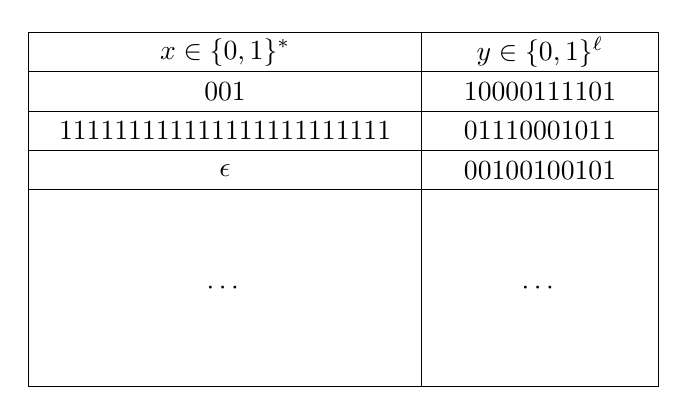
\begin{tikzpicture}[auto, node distance=2.5cm,>=latex']
		\draw (0,0) rectangle (8,0.5);
		\draw (0,0) rectangle (8,-4);
		\draw (5,0.5) -- (5,-4);
		\draw (0,-0.5) -- (8,-0.5);
		\draw (0,-1) -- (8,-1);
		\draw (0,-1.5) -- (8,-1.5);

		\node at (2.5, 0.25) {$x \in \{0, 1\}^*$};
		\node at (2.5, -0.25) {$001$};
		\node at (6.5, 0.25) {$y \in \{0, 1\}^\ell$};
		\node at (6.5, -0.25) {$10000111101$};
		\node at (2.5, -0.75) {$111111111111111111111111$};
		\node at (6.5, -0.75) {$01110001011$};
		\node at (2.5, -1.25) {$\epsilon$};
		\node at (6.5, -1.25) {$00100100101$};

		\node at (2.5, -2.75) {$\cdots$};
		\node at (6.5, -2.75) {$\cdots$};
	\end{tikzpicture}
	\begin{itemize}
		\item The table is initially empty.
		\item When query $x \in \Sigma^*$, if $x$ is in left part, returns the corresponding $y$; otherwise return a random $y \in_R \{0, 1\}^\ell$ and writes $(x, y)$ into table.
	\end{itemize}
\end{frame}

\end{document}